\documentclass[11pt,a4paper]{article}

\usepackage[T1]{fontenc}
\usepackage[utf8]{inputenc}
\usepackage{amsmath,amsthm}
\usepackage{newtxtext,newtxmath}
\usepackage[varqu]{zi4}
\usepackage{microtype}
\usepackage[margin=1in]{geometry}
\usepackage{array,booktabs,tabularx}
\usepackage[dvipsnames]{xcolor}
\usepackage{tikz}
\usetikzlibrary{positioning,arrows.meta,shapes.geometric,calc,fit,backgrounds,decorations.pathreplacing}
\usepackage{pgfplots}
\pgfplotsset{compat=1.18}
\usepackage{listings}
\usepackage[most]{tcolorbox}
\usepackage[font=small,labelfont=bf]{caption}
\usepackage{enumitem}
\usepackage[colorlinks,linkcolor=MidnightBlue,citecolor=MidnightBlue,urlcolor=MidnightBlue]{hyperref}
\usepackage[nameinlink]{cleveref}

% ---------------------------------------------------------------- notation
\newcommand{\cmb}[1]{\textsf{#1}}
\newcommand{\I}{\cmb{I}}
\newcommand{\K}{\cmb{K}}
\newcommand{\Sc}{\cmb{S}}
\newcommand{\B}{\cmb{B}}
\newcommand{\C}{\cmb{C}}
\newcommand{\Sp}{\cmb{S}'}
\newcommand{\Bs}{\cmb{B}^{*}}
\newcommand{\Cp}{\cmb{C}'}
\newcommand{\Y}{\cmb{Y}}
\newcommand{\IF}{\cmb{IF}}
\newcommand{\abs}[2]{[#1]\,#2}
\newcommand{\red}{\;\to\;}
\newcommand{\reds}{\;\to^{*}\;}

% graph = blue, spine = green, code = orange, heap = purple
\definecolor{tfill}{HTML}{DCE9F7}
\definecolor{sfill}{HTML}{DDF0DC}
\definecolor{cfill}{HTML}{FCE8D2}
\definecolor{hfill}{HTML}{F1DDEE}
\definecolor{tline}{HTML}{2F6DB5}
\definecolor{sline}{HTML}{3C8A3A}
\definecolor{cline}{HTML}{C7701C}
\definecolor{hline}{HTML}{9A3F8E}

\tikzset{
  >=Stealth,
  every picture/.append style={font=\small},
  ptr/.style={->, thick},
  half/.style={draw, minimum width=0.62cm, minimum height=0.55cm, inner sep=1pt, fill=white, font=\small\sffamily},
  newhalf/.style={half, fill=cfill},
  rooth/.style={half, fill=tfill},
  leaf/.style={inner sep=1.5pt, font=\small\sffamily},
  scell/.style={draw=sline, fill=sfill, minimum width=0.9cm, minimum height=0.5cm, font=\footnotesize, inner sep=1pt},
}
% \gcell[style]{name}{position}{fun}{arg}: an application cell of two halves,
% name-f and name-a
\newcommand{\gcell}[5][half]{%
  \node[#1, anchor=east] (#2-f) at (#3) {#4};
  \node[#1, anchor=west] (#2-a) at (#3) {#5};}

\theoremstyle{definition}
\newtheorem{definition}{Definition}
\newtheorem{exercise}{Exercise}
\theoremstyle{plain}
\newtheorem{theorem}{Theorem}

\newtcolorbox{aside}[1]{enhanced, breakable, colback=black!3, colframe=black!35,
  boxrule=0.5pt, arc=2pt, fonttitle=\bfseries\small, title={#1}, coltitle=black,
  colbacktitle=black!10, left=6pt, right=6pt}

\lstdefinelanguage{vm16}{morekeywords={LI,MOV,LW,SW,LB,SB,LWA,SWA,ADD,SUB,AND,OR,XOR,MUL,DIVU,
  NOT,NEG,SHL,SHR,SAR,ADDI,BEQ,BNE,BLT,BGE,BLTU,BGEU,BZ,BNZ,JMP,JR,PUSH,POP,GETDSP,SETDSP,
  GETRSP,CALL,CALLR,RET,SYS,HALT},
  sensitive=true, morecomment=[l]{;}}
\lstset{language=vm16, basicstyle=\ttfamily\small, keywordstyle=\bfseries,
  commentstyle=\color{black!55}, columns=fullflexible, keepspaces,
  frame=single, rulecolor=\color{black!30}, xleftmargin=6pt, xrightmargin=6pt,
  aboveskip=8pt, belowskip=8pt, tabsize=8}
\lstdefinestyle{plain}{language={}, keywordstyle={}}

\title{Combinator Graph Reduction\\[4pt]\large A Tutorial Introduction}
\author{}
\date{\today}

\begin{document}
\maketitle

\begin{abstract}
\noindent
In 1979 David Turner showed that a functional program can be run without
environments, closures or variables of any kind. The program is first
translated into a handful of \emph{combinators}, fixed functions such as
$\Sc$, $\K$ and $\I$, by a process called bracket abstraction. The result is a
tree of applications, which a very simple machine then rewrites, one
combinator at a time, until a value remains. Because the tree is rewritten in
place, and subtrees are shared rather than copied, it becomes a
\emph{graph}, and the machine evaluates lazily: an argument is evaluated only
when it is needed, and then only once. This tutorial develops the technique
from the beginning. It shows how bracket abstraction works and why Turner's
extra combinators make it practical, how the reduction machine finds and
rewrites redexes, and how recursion becomes a cycle in the graph. It traces
small programs step by step, shows what laziness buys (conditionals without
thunks, infinite lists) and what it costs, and then looks at a complete
implementation on the VM16 virtual machine with a copying garbage collector,
measured against the SECD machine and the Categorical Abstract Machine. The
prerequisites are the untyped $\lambda$-calculus and, ideally, the companion
tutorials on the SECD machine and the CAM.
\end{abstract}

\tableofcontents

% =====================================================================
\section{Introduction}

The SECD machine~\cite{landin64} and the Categorical Abstract Machine
(CAM)~\cite{cam87} evaluate $\lambda$-terms in much the same way. Both keep an
\emph{environment} that tells them the value of each variable, both build
\emph{closures} that pair a function's code with the environment it was
defined in, and both evaluate an argument before passing it to a function.
The first two are the price of having variables; the third is a choice.

In 1979 David Turner described a different way~\cite{turner79}. If a program
contains no variables, it needs no environments and no closures. And any
$\lambda$-term can be translated into a term without variables, built only
from a few fixed functions called \emph{combinators}. The idea goes back to
Schönfinkel~\cite{schonfinkel24} and Curry~\cite{curryfeys58}, who showed in
the 1920s and 1930s that two combinators, $\Sc$ and $\K$, are enough to
express every $\lambda$-term. Turner's contributions were a translation that
produces reasonably small code, and an efficient way to run it: represent the
program as a graph of application nodes and \emph{rewrite} the graph, one
combinator at a time, until a value is left.

Turner used the technique to implement his languages SASL and KRC, and later
Miranda, the most direct ancestor of Haskell. It has three attractive
properties.

\begin{enumerate}[itemsep=2pt]
\item \textbf{The machine is tiny.} Each combinator is a fixed rewrite rule,
  such as $\Sc\,f\,g\,x \red f\,x\,(g\,x)$. The whole machine is a loop that
  finds the next combinator to apply and rewrites the graph according to its
  rule. Cambridge researchers built it in hardware, as SKIM~\cite{skim80}.
\item \textbf{Evaluation is lazy for free.} Rewriting a shared node in place
  means that every part of the program that refers to it sees the result.
  So an argument is evaluated at most once, and only if it is needed:
  call-by-need, or \emph{lazy evaluation}, without any extra machinery.
\item \textbf{Recursion is a cycle.} The fixpoint combinator $\Y$ can be
  implemented by making a node point to itself, so a recursive function
  costs nothing per call to set up.
\end{enumerate}

The price is that programs take many small steps, and that the translation
can make them large. We will measure both.

\paragraph{Plan.} \Cref{sec:combinators} introduces combinators and
\cref{sec:abstraction} the translation into them, bracket abstraction, with
Turner's improvements. \Cref{sec:graphs} explains why the program is a graph
and not a tree, and \cref{sec:machine} gives the reduction machine.
\Cref{sec:examples} traces programs through it, \cref{sec:recursion} adds
conditionals and recursion, and \cref{sec:laziness} looks at laziness, for
better and worse. \Cref{sec:vm16} describes an implementation on the VM16
virtual machine and \cref{sec:measure} measures it. The paper ends with the
descendants of the technique, exercises and a reference card.

\paragraph{Notation.} We use the language of the companion tutorials:
single-letter variables, $\lambda x\,y.M$ for $\lambda x.\lambda y.M$,
application associating to the left, 15-bit integers, and curried operators
written in prefix form, as in ${-}\;n\;1$ for $n-1$. The implementation reads
the same syntax, with \verb|\| for $\lambda$.

% =====================================================================
\section{Combinators}\label{sec:combinators}

A \emph{combinator} is a $\lambda$-term without free variables. A few of them
are useful enough to have names:

\begin{center}
\begin{tabular}{@{}l l l@{}}
\toprule
combinator & definition & rewrite rule\\
\midrule
$\I$ & $\lambda x.\,x$ & $\I\,x \red x$\\
$\K$ & $\lambda x\,y.\,x$ & $\K\,x\,y \red x$\\
$\Sc$ & $\lambda f\,g\,x.\,f\,x\,(g\,x)$ & $\Sc\,f\,g\,x \red f\,x\,(g\,x)$\\
\bottomrule
\end{tabular}
\end{center}

\noindent
$\I$ is the identity, and $\K$ makes constant functions: $\K\,x$ is the
function that ignores its argument and returns $x$. $\Sc$ is less obvious.
It takes two functions and an argument, gives the argument to both, and
applies the first result to the second. We will see in the next section that
$\Sc$ is exactly what is needed to push an argument down into both halves of
an application.

\begin{definition}
A \emph{combinator term} is built from combinators, constants and
application, with no $\lambda$s and no variables. A combinator applied to as
many arguments as its rule needs is a \emph{redex}, and replacing it by the
right-hand side of its rule is a \emph{reduction}.
\end{definition}

Reduction never needs to substitute anything: the rules only rearrange their
arguments. That is the point. For example, $\Sc\,\K\,\K$ behaves like $\I$:
\[
  \Sc\,\K\,\K\,x \red \K\,x\,(\K\,x) \red x.
\]
So $\I$ is not even needed; $\Sc$ and $\K$ suffice, a fact due to
Schönfinkel~\cite{schonfinkel24}. A machine for combinator terms needs no
environment, because there is nothing to look up, and no closures, because
there is nothing to capture. It only has to find redexes and rewrite them.

% =====================================================================
\section{Bracket abstraction}\label{sec:abstraction}

\subsection{The basic algorithm}

How do we get rid of the $\lambda$s? The trick is to eliminate one variable at
a time. Write $\abs{x}{e}$ for a term without $x$ such that
\[
  (\abs{x}{e})\;x \reds e.
\]
$\abs{x}{e}$ behaves like $\lambda x.e$, but it is built from combinators. If
$e$ itself contains no $\lambda$s, three cases suffice:
\begin{align*}
  \abs{x}{x} &= \I\\
  \abs{x}{e} &= \K\,e \qquad\text{if $e$ is a constant, a combinator or a variable other than $x$}\\
  \abs{x}{(e_1\;e_2)} &= \Sc\;(\abs{x}{e_1})\;(\abs{x}{e_2})
\end{align*}
The third case is where $\Sc$ comes in. Applying the right-hand side to $x$
gives $(\abs{x}{e_1})\,x\;((\abs{x}{e_2})\,x)$ by the rule for $\Sc$, and each
half then turns back into $e_1$ and $e_2$.

To compile a whole program, we work from the inside out: for each $\lambda x.M$,
first compile $M$, which removes the $\lambda$s inside it, then abstract $x$
from the result.

\begin{theorem}\label{thm:abs}
If $e$ contains no $\lambda$s, then $\abs{x}{e}$ contains no $x$, and
$(\abs{x}{e})\;x \reds e$.
\end{theorem}

\begin{proof}
By induction on $e$. For $x$, $\I\,x \red x$. For any other leaf $e$,
$\K\,e\,x \red e$. For an application,
$\Sc\,(\abs{x}{e_1})\,(\abs{x}{e_2})\,x \red (\abs{x}{e_1})\,x\,((\abs{x}{e_2})\,x)$,
and by induction the two parts reduce to $e_1$ and $e_2$. None of the
right-hand sides introduces $x$.
\end{proof}

\subsection{An example}

Take $\lambda x\,y.\,y\,x$, which applies its second argument to its first.
The inner abstraction comes first:
\begin{align*}
  \abs{y}{(y\;x)} &= \Sc\;(\abs{y}{y})\;(\abs{y}{x}) = \Sc\;\I\;(\K\,x).
\end{align*}
Now abstract $x$ from that:
\begin{align*}
  \abs{x}{(\Sc\;\I\;(\K\,x))}
  &= \Sc\;(\abs{x}{(\Sc\;\I)})\;(\abs{x}{(\K\,x)})\\
  &= \Sc\;(\Sc\;(\K\,\Sc)\;(\K\,\I))\;(\Sc\;(\K\,\K)\;\I).
\end{align*}
That is correct, but it is a lot of code for such a small function: 9
application cells. Two improvements bring it down to 1.

\subsection{Turner's combinators}\label{sec:turner}

The $\Sc$ rule passes $x$ to both halves of an application, even when only
one half needs it. Turner~\cite{turner79,turner79b} added combinators for the
cases where it does not, and simplified each $\Sc$ as it is built:

\begin{center}
\renewcommand{\arraystretch}{1.15}
\begin{tabular}{@{}l l l@{}}
\toprule
simplification & combinator & meaning\\
\midrule
$\Sc\,(\K\,p)\,(\K\,q) = \K\,(p\,q)$ & & no part needs $x$\\
$\Sc\,(\K\,p)\,\I = p$ & & $\lambda x.\,p\,x$ is $p$ ($\eta$)\\
$\Sc\,(\K\,p)\,q = \B\,p\,q$ & $\B\,f\,g\,x \red f\,(g\,x)$ & only the argument needs $x$\\
$\Sc\,p\,(\K\,q) = \C\,p\,q$ & $\C\,f\,g\,x \red f\,x\,g$ & only the function needs $x$\\
$\Sc\,(\K\,p)\,(\B\,q\,r) = \Bs\,p\,q\,r$ & $\Bs\,k\,f\,g\,x \red k\,(f\,(g\,x))$ & $\B$ inside $\B$\\
$\Sc\,(\B\,p\,q)\,(\K\,r) = \Cp\,p\,q\,r$ & $\Cp\,k\,f\,g\,x \red k\,(f\,x)\,g$ & $\C$ with a function $p$ applied first\\
$\Sc\,(\B\,p\,q)\,r = \Sp\,p\,q\,r$ & $\Sp\,k\,f\,g\,x \red k\,(f\,x)\,(g\,x)$ & $\Sc$ with a function $p$ applied first\\
\bottomrule
\end{tabular}
\end{center}

\noindent
The rules are tried in this order. The first is really the $\K$ case of the
basic algorithm, applied to whole subterms: if neither half contains $x$, the
whole application does not either. $\B$ and $\C$ are the two halves of $\Sc$:
$\B$ routes $x$ only into the argument, $\C$ only into the function. The
\emph{primed} combinators $\Sp$, $\Bs$ and $\Cp$ deal with something that
happens all the time in curried code: a function of several arguments, such
as $\Sc\,(\B\,p\,q)\,r$, where the first combinator only exists to apply $p$
to the result. They do the same job with one cell fewer and one reduction
fewer.

With these rules, the example becomes:
\begin{align*}
  \abs{y}{(y\;x)} &= \Sc\;\I\;(\K\,x) = \C\;\I\;x\\
  \abs{x}{(\C\;\I\;x)} &= \Sc\;(\K\,(\C\,\I))\;\I = \C\;\I.
\end{align*}
One cell. And indeed $\C\,\I\,a\,f \red \I\,f\,a \red f\,a$.

\Cref{tab:abs} shows more examples, as printed by the implementation, which
compiles a program and prints the result if it is preceded by \texttt{?}.

\begin{table}[t]
\centering
\small
\begin{tabular}{@{}l l l@{}}
\toprule
$\lambda$-term & with $\Sc$, $\K$, $\I$ only & with Turner's rules\\
\midrule
$\lambda x\,y.\,x$ & $\Sc\,(\K\,\K)\,\I$ & $\K$\\
$\lambda x\,y.\,y\,x$ & $\Sc\,(\K\,(\Sc\,\I))\,(\Sc\,(\K\,\K)\,\I)$ & $\C\,\I$\\
$\lambda x.\,{+}\;x\;1$ & $\Sc\,(\Sc\,(\K\,{+})\,\I)\,(\K\,1)$ & $\C\,{+}\,1$\\
$\lambda x.\,x\,x$ & $\Sc\,\I\,\I$ & $\Sc\,\I\,\I$\\
$\lambda f\,x.\,f\,(f\,x)$ & $\Sc\,(\Sc\,(\K\,\Sc)\,(\Sc\,(\K\,\K)\,\I))\,(\Sc\,(\Sc\,(\K\,\Sc)\,(\Sc\,(\K\,\K)\,\I))\,(\K\,\I))$ & $\Sc\,\B\,\I$\\
\bottomrule
\end{tabular}
\caption{Bracket abstraction with and without Turner's rules. The plain
algorithm here already includes the rule
$\Sc\,(\K\,p)\,(\K\,q) = \K\,(p\,q)$, which is why $\abs{x}{(\Sc\,\I)}$ in the
second line became $\K\,(\Sc\,\I)$.}
\label{tab:abs}
\end{table}

\begin{aside}{How large can the code get?}
Each abstraction can make a term up to three times larger, and nested
abstractions compound: with the three basic rules alone, code can grow
exponentially with the nesting depth of $\lambda$s. The $\K$ simplification
avoids that, but the worst case remains quadratic in the size of the
program, even with Turner's rules. Algorithms with a linear worst case exist;
they use whole families of combinators, such as $\B_n$ and $\C_n$ for
routing an argument past $n$ others. Kiselyov~\cite{kiselyov18} gives a
recent and very readable account. For the programs in this tutorial, Turner's
rules shrink the code by a factor of 2.5 to 6 (\cref{tab:sizes}).
\end{aside}

\subsection{Reading compiled code}

Factorial is
\[
  \mathbf{rec}\ f.\ \lambda n.\ \mathbf{if}\ ({=}\ n\ 0)\ 1\ ({*}\ n\ (f\ ({-}\ n\ 1)))
\]
where $\mathbf{rec}\ f.M$ is $\Y\,(\lambda f.M)$ (\cref{sec:recursion}) and
$\mathbf{if}\,c\,t\,e$ is the combinator $\IF$ applied to $c$, $t$ and $e$.
It compiles to a term of 16 cells:
\[
  \Y\;(\Bs\;(\Sc\;(\Cp\;\IF\;(\C\;{=}\;0)\;1))\;(\Sc\;{*})\;(\C\;\B\;(\C\;{-}\;1))).
\]
It can be read piece by piece. $\C\,{=}\,0$ is $\lambda n.\,{=}\;n\;0$, and
$\C\,{-}\,1$ is $\lambda n.\,{-}\;n\;1$. $\C\,\B\,(\C\,{-}\,1)$ takes $f$ and then
$n$ and gives $f\,({-}\;n\;1)$; $\Sc\,{*}$ multiplies $n$ by that; and
$\Cp\,\IF\,(\C\,{=}\,0)\,1$ takes the result as the else-branch and builds the
conditional. $\Bs$ and $\Sc$ distribute $f$ and $n$ to the parts that need
them. Nobody would write it that way, but it needs no variables.

% =====================================================================
\section{From trees to graphs}\label{sec:graphs}

A combinator term is a binary tree of applications. Each application is a
cell with two fields, the function and the argument; the leaves are
combinators and numbers. To reduce $\Sc\,f\,g\,x$, we could build the tree for
$f\,x\,(g\,x)$, with two copies of $x$. But $x$ may be a large unevaluated
expression, and copying it would mean evaluating it twice later.

The solution is not to copy it: both new cells point to the same $x$
(\cref{fig:srule}). From then on the program is a \emph{graph}, in which a
cell can have several parents. This is safe as long as nothing ever changes
the \emph{meaning} of a cell, and the rewrite rules never do. They only
replace a cell's contents by something equal to it.

\begin{figure}[t]
\centering
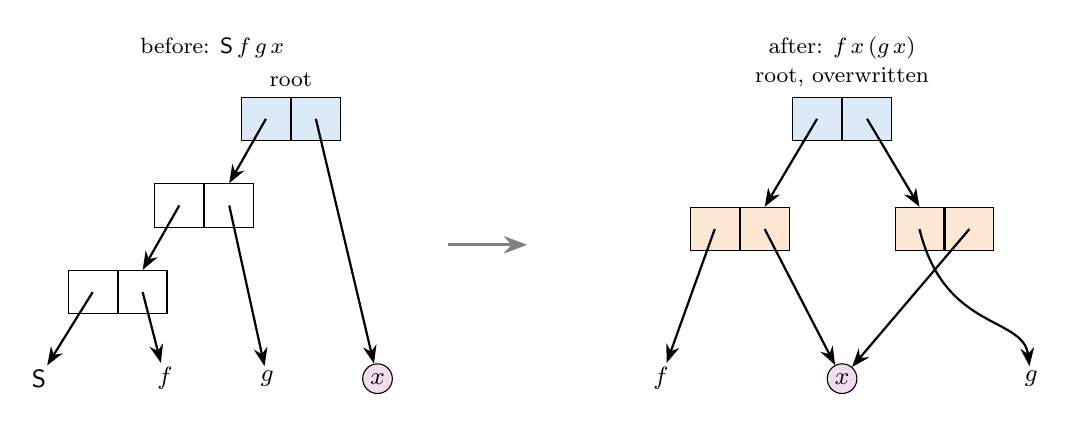
\begin{tikzpicture}[node distance=0.4cm]
% before
\begin{scope}
\gcell[rooth]{r}{0,0}{}{}
\gcell{c2}{-1.1,-1.1}{}{}
\gcell{c1}{-2.2,-2.2}{}{}
\node[leaf] (S) at (-3.2,-3.3) {S};
\node[leaf] (f) at (-1.6,-3.3) {$f$};
\node[leaf] (g) at (-0.3,-3.3) {$g$};
\node[draw, circle, inner sep=1.5pt, fill=hfill] (x) at (1.1,-3.3) {$x$};
\draw[ptr] (r-f.center) -- (c2-a.north);
\draw[ptr] (c2-f.center) -- (c1-a.north);
\draw[ptr] (c1-f.center) -- (S);
\draw[ptr] (c1-a.center) -- (f);
\draw[ptr] (c2-a.center) -- (g);
\draw[ptr] (r-a.center) -- (x);
\node[font=\footnotesize, anchor=south] at (r-f.north east) {root};
\node[font=\footnotesize] at (-1,0.9) {before: $\Sc\,f\,g\,x$};
\end{scope}
\draw[->, very thick, black!50] (2.0,-1.6) -- (3.0,-1.6);
% after
\begin{scope}[xshift=7cm]
\gcell[rooth]{r}{0,0}{}{}
\gcell[newhalf]{p}{-1.3,-1.4}{}{}
\gcell[newhalf]{q}{1.3,-1.4}{}{}
\node[leaf] (f) at (-2.3,-3.3) {$f$};
\node[draw, circle, inner sep=1.5pt, fill=hfill] (x) at (0,-3.3) {$x$};
\node[leaf] (g) at (2.4,-3.3) {$g$};
\draw[ptr] (r-f.center) -- (p-a.north);
\draw[ptr] (r-a.center) -- (q-f.north);
\draw[ptr] (p-f.center) -- (f);
\draw[ptr] (p-a.center) -- (x);
\draw[ptr] (q-f.center) .. controls (1.3,-2.7) and (2.3,-2.5) .. (g);
\draw[ptr] (q-a.center) -- (x);
\node[font=\footnotesize, anchor=south] at (r-f.north east) {root, overwritten};
\node[font=\footnotesize] at (0,0.9) {after: $f\,x\,(g\,x)$};
\end{scope}
\end{tikzpicture}
\caption{The $\Sc$ rule on a graph. Each box pair is an application cell: the
left half points to the function, the right half to the argument. The root
of the redex (blue) is overwritten; two new cells (orange) are allocated; and
$x$ is shared rather than copied. The three old cells of the spine become
garbage unless something else refers to them.}
\label{fig:srule}
\end{figure}

\paragraph{Overwrite the root.} Notice what happened to the root of the
redex, the outermost cell of $\Sc\,f\,g\,x$. The rule does not build a new
cell for $f\,x\,(g\,x)$ and leave the old one alone. It \emph{overwrites} the
root with the new contents. Other parts of the program may point to that
same cell, because it may itself be a shared argument. When it is
overwritten, they all see the reduced version, and none of them will reduce
it again. This is what makes evaluation \emph{lazy} in the full sense,
call-by-need: an expression is reduced only when something needs its value,
and at most once.

\paragraph{Indirections.} Sometimes the result is not an application. After
$\K\,x\,y \red x$, the root should become $x$ itself, but if $x$ is a number
or a combinator, it does not fit in a cell, and if $x$ is a cell, copying its
two fields into the root would duplicate it, losing sharing. The standard
answer is to overwrite the root with $\I\,x$, an \emph{indirection}. Anything
that reaches the root then finds $\I\,x$ and goes on to $x$. In this machine
an indirection is not a special kind of cell: it is just an ordinary $\I$
redex, and reducing it is an ordinary reduction.

% =====================================================================
\section{The reduction machine}\label{sec:machine}

\subsection{Finding the next redex}

Lazy evaluation reduces the \emph{leftmost outermost} redex first: the one
at the head of the whole expression. To find it, the machine walks down the
left-hand, \emph{function} fields from the root, remembering every cell it
passes, until it reaches a leaf. This path is the \emph{spine}, and the walk
is called \emph{unwinding}. The cells of the spine are kept on a stack, with
the innermost on top. \Cref{fig:spine} shows the spine of
$\C\;{+}\;1\;41$.

\begin{figure}[t]
\centering
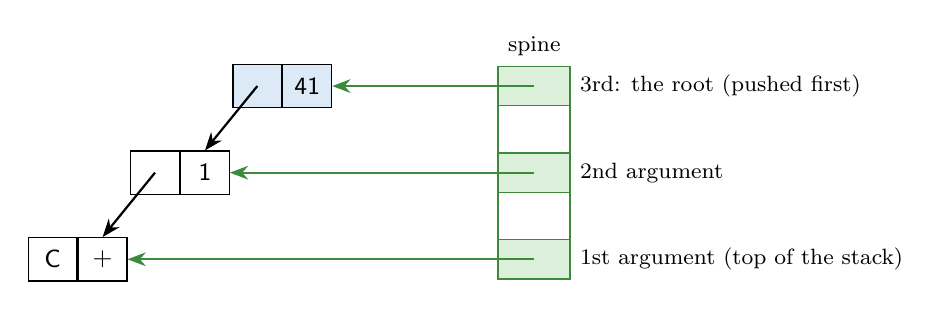
\begin{tikzpicture}
\gcell[rooth]{r}{0,0}{}{41}
\gcell{c2}{-1.3,-1.1}{}{1}
\gcell{c1}{-2.6,-2.2}{C}{+}
\draw[ptr] (r-f.center) -- (c2-a.north);
\draw[ptr] (c2-f.center) -- (c1-a.north);
% spine stack, growing down as the VM16 data stack does
\node[scell] (s3) at (3.2,0) {};
\node[scell] (s2) at (3.2,-1.1) {};
\node[scell] (s1) at (3.2,-2.2) {};
\draw[sline, thick] (s3.north west) -- (s1.south west) (s3.north east) -- (s1.south east);
\node[font=\footnotesize, anchor=south] at (s3.north) {spine};
\node[font=\footnotesize, anchor=west] at (s3.east) {3rd: the root (pushed first)};
\node[font=\footnotesize, anchor=west] at (s2.east) {2nd argument};
\node[font=\footnotesize, anchor=west] at (s1.east) {1st argument (top of the stack)};
\draw[ptr, sline] (s1.center) -- (c1-a.east);
\draw[ptr, sline] (s2.center) -- (c2-a.east);
\draw[ptr, sline] (s3.center) -- (r-a.east);
\end{tikzpicture}
\caption{Unwinding $\C\;{+}\;1\;41$. The machine follows function fields from
the root down to the combinator $\C$, pushing each cell. The argument of the
$i$th cell from the top is the $i$th argument of $\C$, and the 3rd cell is
the root of the redex, because $\C$ takes three arguments.}
\label{fig:spine}
\end{figure}

When the walk ends at a leaf, there are three cases:

\begin{itemize}[itemsep=2pt]
\item \textbf{A combinator with enough arguments.} If the combinator needs
  $n$ arguments and the spine has at least $n$ cells, the top $n$ cells hold
  the arguments, in their argument fields, and the $n$th is the root of the
  redex. The machine applies the rule, overwrites the root, pops the $n$
  cells, and unwinds again from the root.
\item \textbf{A combinator with too few arguments.} Then the expression is a
  partial application such as ${+}\;3$. It cannot be reduced further: it is
  in \emph{weak head normal form} (WHNF), and the machine stops.
\item \textbf{A number.} If the spine is empty, the number is the result. If
  not, the program tried to apply a number to an argument, which is an error.
\end{itemize}

\noindent
Note that after a rewrite the machine continues from the root of the redex,
not from the top of the whole program. The cells below the root on the stack
are still on the spine, and nothing above them has changed.

\subsection{The rules}\label{sec:rules}

\Cref{fig:rules} lists every rule. The combinator rules only rearrange
pointers; the rules for $\IF$ and the arithmetic operators are different,
because they need the \emph{values} of some arguments. To get the value of
an argument $a$, the machine runs itself recursively on $a$, with a new spine
on top of the old one, until $a$ is in WHNF. Because the graph is updated in
place, the argument cell now holds its value (or an indirection to it), for
the benefit of anyone else who refers to it.

\begin{figure}[t]
\centering
\small
\renewcommand{\arraystretch}{1.2}
\begin{tabular}{@{}l l l@{}}
\toprule
rule & new cells & what the root becomes\\
\midrule
$\I\,x \red x$ & 0 & (the parent is pointed at $x$ directly)\\
$\K\,x\,y \red x$ & 0 & $\I\,x$\\
$\Sc\,f\,g\,x \red f\,x\,(g\,x)$ & 2 & $(f\,x)\;(g\,x)$\\
$\B\,f\,g\,x \red f\,(g\,x)$ & 1 & $f\;(g\,x)$\\
$\C\,f\,g\,x \red f\,x\,g$ & 1 & $(f\,x)\;g$\\
$\Sp\,k\,f\,g\,x \red k\,(f\,x)\,(g\,x)$ & 3 & $(k\,(f\,x))\;(g\,x)$\\
$\Bs\,k\,f\,g\,x \red k\,(f\,(g\,x))$ & 2 & $k\;(f\,(g\,x))$\\
$\Cp\,k\,f\,g\,x \red k\,(f\,x)\,g$ & 2 & $(k\,(f\,x))\;g$\\
$\Y\,f \red f\,(\Y\,f)$ & 0 & $f\;\text{root}$: the root points to itself\\
$\IF\,c\,t\,e \red t$ or $e$ & 0 & $\I\,t$ if $c \ne 0$, else $\I\,e$, after reducing $c$\\
${+}\,a\,b \red a+b$ & 0 & $\I\,(a+b)$, after reducing $a$ and $b$; likewise ${-}\ {*}\ {/}\ {\%}\ {=}\ {<}$\\
\bottomrule
\end{tabular}
\caption{The rewrite rules. ``New cells'' counts the cells allocated; the root
of the redex is always reused. $\IF$ and the operators reduce some
arguments first, by a recursive call of the machine.}
\label{fig:rules}
\end{figure}

\paragraph{Short-circuiting indirections.} When the machine reduces
$\I\,x$, it also changes the parent cell on the spine, if there is one, to
point at $x$ instead of at the indirection. This is free (one store), and it
means an indirection is usually passed through only once. The same happens
after $\K$, $\IF$ and the operators, which leave an indirection behind in the
root: the parent is pointed straight at the result.

\subsection{Weak head normal form, and printing}

The machine stops at WHNF: a number, or a function still waiting for
arguments. It does not reduce inside a partial application, so
$\lambda x.\,{+}\;1\;2$ is not simplified to a constant function of 3 until it
is applied. That is the same choice the SECD machine and the CAM make when
they stop at a closure, and for the same reason: the inside of a function
only matters when it is called. The implementation prints a number as a
number and anything else as \verb|<function>|.

% =====================================================================
\section{Worked examples}\label{sec:examples}

The traces in this section were produced by \texttt{prototype.py
-{}-trace}, a Python model of the implementation that makes exactly the same
reductions in the same order. Each line shows the whole program graph after
one more reduction, written as a term, so a shared cell appears once for each
of its parents. Indirections are shown as $\I\,x$.

\subsection{A function call}

$(\lambda x.\,{+}\;x\;1)\;41$ compiles to $\C\;{+}\;1\;41$ (\cref{tab:abs}),
and runs in two reductions:

\begin{center}
\small
\begin{tabular}{@{}r l l@{}}
\toprule
step & rule & graph\\
\midrule
0 & & $\C\;{+}\;1\;41$\\
1 & $\C$ & ${+}\;41\;1$\\
2 & ${+}$ & $\I\;42$\\
\bottomrule
\end{tabular}
\end{center}

\noindent
After step 1, unwinding the root finds ${+}$ with two arguments. The machine
evaluates $41$ and $1$ (both are already numbers) and overwrites the root
with $\I\,42$; with no parent to update, the machine continues at $42$, an
empty spine and a number, so it stops. The CAM needed 13 instructions for the
same program.

\subsection{Sharing: twice}

$\lambda f\,x.\,f\,(f\,x)$ compiles to $\Sc\,\B\,\I$. Applied to ${+}\;1$
and $0$, it shows the first sharing:

\begin{center}
\small
\begin{tabular}{@{}r l l@{}}
\toprule
step & rule & graph\\
\midrule
0 & & $\Sc\;\B\;\I\;({+}\;1)\;0$\\
1 & $\Sc$ & $\B\;({+}\;1)\;(\I\;({+}\;1))\;0$\\
2 & $\B$ & ${+}\;1\;(\I\;({+}\;1)\;0)$\\
3 & $\I$ & ${+}\;1\;({+}\;1\;0)$\\
4 & ${+}$ & ${+}\;1\;(\I\;1)$\\
5 & ${+}$ & $\I\;2$\\
\bottomrule
\end{tabular}
\end{center}

\noindent
At step 1, $\Sc$ gives its third argument, ${+}\;1$, to both $\B$ and $\I$.
The two occurrences in the line are the same cell. At step 4, the outer
${+}$ needs the value of its second argument, so the machine calls itself on
the cell ${+}\;1\;0$, which is overwritten with $\I\,1$. Step 3 was
an $\I$ reduction that the compiler put there: $\Sc\,\B\,\I$ uses $\I$ to say
``and pass $f$ unchanged''.

\subsection{Laziness}

$(\lambda x\,y.\,y)\;({/}\;1\;0)\;5$ compiles to $\K\;\I\;({/}\;1\;0)\;5$.
$\K$ discards its second argument, so the division by zero is never
attempted:

\begin{center}
\small
\begin{tabular}{@{}r l l@{}}
\toprule
step & rule & graph\\
\midrule
0 & & $\K\;\I\;({/}\;1\;0)\;5$\\
1 & $\K$ & $\I\;5$\\
2 & $\I$ & $\I\;5$\\
\bottomrule
\end{tabular}
\end{center}

\noindent
After step 1, the root of the $\K$ redex is the cell $\K\,\I\,({/}\,1\,0)$,
which becomes $\I\,\I$; its parent, the program root, is pointed straight at
$\I$, so the program reads $\I\,5$. Step 2 reduces that, and the machine
stops at 5. On the SECD machine and the CAM, the same program fails with
``division by zero''.

% =====================================================================
\section{Conditionals and recursion}\label{sec:recursion}

\subsection{IF without thunks}

The companion tutorials spend some time on conditionals. In a strict machine,
$\mathit{cond}\;c\;t\;e$ written as an ordinary function evaluates both $t$
and $e$ before choosing one, so a recursive function such as factorial never
stops. The SECD tutorial wraps each branch in $\lambda d.$ and applies the
chosen one to a dummy argument, and both machines also get a special
\textbf{if} form that evaluates only one branch.

In a lazy machine none of this is needed. $\IF$ is an ordinary combinator of
three arguments, and the rule for it reduces only the condition. The branch
it does not choose is never touched. Even Church booleans,
$\lambda x\,y.\,x$ and $\lambda x\,y.\,y$, work as conditionals: they compile
to $\K$ and $\K\,\I$, and only the chosen argument is ever reduced. $\IF$ is
just faster.

\subsection{Recursion as a cycle}

$\mathbf{rec}\ f.M$ means $M$, where $f$ refers to $M$ itself. The compiler
turns it into $\Y\,(\lambda f.M)$, where $\Y$ is the fixpoint combinator,
$\Y\,h = h\,(\Y\,h)$. As a $\lambda$-term, $\Y$ has to make a copy of
$h\,(\Y\,h)$ each time the recursion unfolds. In a graph, it can do better.
The rule overwrites the root, the cell $\Y\,h$, with $h$ applied to
\emph{the root itself} (\cref{fig:ycycle}). The result is a cycle in the
graph: the function's own definition is reachable from inside it. Every
recursive call then follows the cycle back, and no further copying is ever
needed. A recursive definition costs one reduction for the whole run.

\begin{figure}[t]
\centering
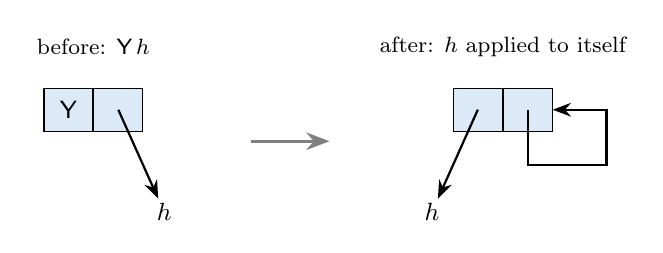
\begin{tikzpicture}
\begin{scope}
\gcell[rooth]{r}{0,0}{Y}{}
\node[leaf] (h) at (0.9,-1.3) {$h$};
\draw[ptr] (r-a.center) -- (h);
\node[font=\footnotesize] at (0,0.8) {before: $\Y\,h$};
\end{scope}
\draw[->, very thick, black!50] (2.0,-0.4) -- (3.0,-0.4);
\begin{scope}[xshift=5.2cm]
\gcell[rooth]{r}{0,0}{}{}
\node[leaf] (h) at (-0.9,-1.3) {$h$};
\draw[ptr] (r-f.center) -- (h);
\draw[ptr] (r-a.center) -- ++(0,-0.7) -- ++(1.0,0) |- (r-a.east);
\node[font=\footnotesize] at (0,0.8) {after: $h$ applied to itself};
\end{scope}
\end{tikzpicture}
\caption{The $\Y$ rule. The root is overwritten with $h$ applied to the root
itself. Unfolding the recursion never copies anything.}
\label{fig:ycycle}
\end{figure}

\paragraph{rec does not need a function.} Since nothing about the cycle
requires $M$ to be a function, $\mathbf{rec}\ l.\,\lambda c\,n.\,c\;1\;l$ is
an infinite list of ones (lists are introduced in \cref{sec:laziness}),
represented by a single cycle. The CAM's \textbf{rec} must be applied to a
$\lambda$; here it can define any value in terms of itself. A definition with
no content, $\mathbf{rec}\ x.\,x$, becomes $\Y\,\I$, then a cell that is an
indirection to itself; the implementation recognises that case and reports
``a value defined as itself'' instead of looping.

\subsection{Factorial}

\Cref{tab:fac} traces factorial applied to 1. Step 1 builds the cycle, shown
as $@$ where the line refers back to the cell being printed. Steps 2 to 7
distribute $n$ and $f$, test $n = 0$, and choose the else-branch. Steps 8 to
12 do the same for the recursive call.

\begin{table}[t]
\centering
\footnotesize
\setlength{\tabcolsep}{4pt}
\begin{tabular}{@{}r l l@{}}
\toprule
step & rule & graph (with $F = \Sc\,(\Cp\,\IF\,(\C\,{=}\,0)\,1)$)\\
\midrule
0 & & $\Y\;(\Bs\;F\;(\Sc\;{*})\;(\C\;\B\;(\C\;{-}\;1)))\;1$\\
1 & $\Y$ & $\Bs\;F\;(\Sc\;{*})\;(\C\;\B\;(\C\;{-}\;1))\;@\;1$\\
2 & $\Bs$ & $F\;(\Sc\;{*}\;(\C\;\B\;(\C\;{-}\;1)\;@))\;1$\\
3 & $\Sc$ & $\Cp\;\IF\;(\C\;{=}\;0)\;1\;1\;(\Sc\;{*}\;(\C\;\B\;(\C\;{-}\;1)\;\ldots)\;1)$\\
4 & $\Cp$ & $\IF\;(\C\;{=}\;0\;1)\;1\;(\Sc\;{*}\;\ldots\;1)$\\
5 & $\C$ & $\IF\;({=}\;1\;0)\;1\;(\Sc\;{*}\;\ldots\;1)$\\
6 & ${=}$ & $\IF\;(\I\;0)\;1\;(\Sc\;{*}\;\ldots\;1)$\\
7 & $\IF$ & $\I\;(\Sc\;{*}\;(\C\;\B\;(\C\;{-}\;1)\;\ldots)\;1)$\\
8 & $\Sc$ & $\I\;({*}\;1\;(\C\;\B\;(\C\;{-}\;1)\;\ldots\;1))$\\
9 & $\C$ & $\I\;({*}\;1\;(\B\;\ldots\;(\C\;{-}\;1)\;1))$\\
10 & $\B$ & $\I\;({*}\;1\;(F\;\ldots\;(\C\;{-}\;1\;1)))$\\
11 & $\Sc$ & $\I\;({*}\;1\;(\Cp\;\IF\;(\C\;{=}\;0)\;1\;(\C\;{-}\;1\;1)\;(\ldots\;(\C\;{-}\;1\;1))))$\\
12 & $\Cp$ & $\I\;({*}\;1\;(\IF\;(\C\;{=}\;0\;(\C\;{-}\;1\;1))\;1\;(\ldots\;(\C\;{-}\;1\;1))))$\\
13 & $\C$ & $\I\;({*}\;1\;(\IF\;({=}\;(\C\;{-}\;1\;1)\;0)\;1\;(\ldots\;(\C\;{-}\;1\;1))))$\\
14 & $\C$ & $\I\;({*}\;1\;(\IF\;({=}\;({-}\;1\;1)\;0)\;1\;(\ldots\;({-}\;1\;1))))$\\
15 & ${-}$ & $\I\;({*}\;1\;(\IF\;({=}\;(\I\;0)\;0)\;1\;(\ldots\;(\I\;0))))$\\
16 & ${=}$ & $\I\;({*}\;1\;(\IF\;(\I\;1)\;1\;(\ldots\;(\I\;0))))$\\
17 & $\IF$ & $\I\;({*}\;1\;(\I\;1))$\\
18 & ${*}$ & $\I\;(\I\;1)$\\
\bottomrule
\end{tabular}
\caption{$(\mathbf{rec}\ f.\,\lambda n.\,\mathbf{if}\,({=}\,n\,0)\,1\,({*}\,n\,(f\,({-}\,n\,1))))\;1$,
abridged from \texttt{prototype.py -{}-trace}: ``$\ldots$'' stands for parts of
the cyclic function that do not change. Steps 13 to 15 show sharing: the
argument $n-1$ of the recursive call is one cell, used both by the test and
by the multiplication, so it is computed once.}
\label{tab:fac}
\end{table}

Two things are worth noticing. First, the argument of the recursive call,
$\C\,{-}\,1\,1$, which is $n - 1$, appears twice in line 12: once in the test
and once in the else-branch. They are the same cell. At step 14 it is
rewritten to ${-}\;1\;1$, and both occurrences change; at step 15 it is
reduced to $\I\,0$, and both see the value. Without sharing, $n-1$ would be
computed twice in every call.

Second, steps 7 and 17 show how the machine handles a conditional in tail
position: $\IF$ replaces its root with an indirection to the chosen branch
and continues there, with no recursive call of the machine. Only the
multiplication, which needs the value of the recursive call, nests. That is
why factorial of $n$ nests $n$ levels deep, while a loop whose recursive call
is the whole result runs in constant stack space (\cref{sec:leaks}).

Factorial of 7 takes 90 reductions, against 171 instructions on the CAM.

% =====================================================================
\section{Laziness, for better and worse}\label{sec:laziness}

\subsection{Infinite lists}

Lazy evaluation makes it possible to define infinite data and use only the
part that is needed. Our language has no built-in lists, but they are easy
to encode as functions. A list is a function of two arguments, what to do with
a non-empty list and what to give for the empty one:
\begin{align*}
  \mathit{cons}\;h\;t &= \lambda c\,n.\,c\;h\;t &
  \mathit{nil} &= \lambda c\,n.\,n.
\end{align*}
To use a list $l$, apply it to a function of the head and tail, and to a
default: $l\;(\lambda h\,t.\,\ldots)\;d$. With these, the integers from $n$ upwards
are
\[
  \mathit{from} = \mathbf{rec}\ f.\,\lambda n.\ \mathit{cons}\ n\ (f\ ({+}\ n\ 1)),
\]
an infinite list. A strict machine would loop forever building it. Here
$\mathit{cons}\;n\;(f\,({+}\,n\,1))$ is in WHNF as soon as $\mathit{cons}$ has
its two arguments: the tail is a graph that has not been reduced, and will
only be reduced if someone asks for it.

The program \texttt{primes.lam} builds on this. It filters multiples out of
$\mathit{from}\;2$ with the sieve of Eratosthenes, getting the infinite list
of primes, and takes element 99:
\begin{lstlisting}[style=plain]
(\C N.                                   # cons, nil
  (\F L.                                 # from, filter
    (\S T.                               # sieve, nth
      T 99 (S (F 2))                     # element 99 (counting from 0)
    )
    (rec s.\l. l (\h t. C h (s (L (\x. % x h) t))) N)
    (rec n.\k l. l (\h t. if (= k 0) h (n (- k 1) t)) 0)
  )
  (rec f.\n. C n (f (+ n 1)))
  (rec g.\p l. l (\h t. if (p h) (C h (g p t)) (g p t)) N)
)
(\h t c n. c h t)
(\c n. n)
\end{lstlisting}
It prints 541 after 155,171 reductions. Only the first 541 integers and the
first 100 primes are ever built. Interestingly, the deepest nesting of the
machine during the run is only 4: almost all of the work is done by $\IF$
choosing a branch and by combinators rearranging pointers, which never nest.

\subsection{Church numerals, as in the textbook}

\texttt{church.lam} computes $5!$ with Church numerals, Church booleans and
the fixpoint combinator $\Y$ written as a $\lambda$-term,
$\lambda f.(\lambda x.f\,(x\,x))\,(\lambda x.f\,(x\,x))$, exactly as a textbook
would write it:
\[
  \Y\;(\lambda f\,n.\ \mathit{iszero}\;n\;\mathit{one}\;(\mathit{times}\;n\;(f\;(\mathit{pred}\;n)))).
\]
Neither the SECD machine nor the CAM can run it: they evaluate the
argument $x\,x$ inside $\Y$, and both branches of the conditional, before
anything else, and recurse forever. (The SECD version, \texttt{fac.lam},
has to use the call-by-value fixpoint combinator $Z$ and wrap each branch in
a $\lambda d.$) Here it gives 120 after 16,957 reductions.

\subsection{Space leaks}\label{sec:leaks}

The flip side of laziness is that unevaluated expressions are kept until
they are needed, and they can pile up. A classic example is a loop with an
accumulator:
\[
  \mathbf{rec}\ f.\,\lambda n\,a.\ \mathbf{if}\ ({=}\ n\ 0)\ a\ (f\ ({-}\ n\ 1)\ ({+}\ a\ 1))
\]
applied to $3000$ and $0$. The test ${=}\;n\;0$ forces $n$ at every step, but
nothing forces $a$. After four rounds the accumulator is the graph
\[
  {+}\;({+}\;({+}\;({+}\;0\;1)\;1)\;1)\;1,
\]
and after 3000 it is a chain of 3000 unevaluated additions. Evaluating it at
the end needs the machine to nest 3000 levels deep, because each ${+}$ needs
the value of the one inside it, and the implementation runs out of stack.
The cure is to force the accumulator on every round, for example by testing
it: with $\mathbf{if}\,({<}\,a\,0)\,0\,(f\,\ldots)$ around the recursive call,
the same loop runs in constant space, in 63,008 reductions. Haskell provides
\texttt{seq} for exactly this purpose (\cref{ex:seq}).

% =====================================================================
\section{An implementation on VM16}\label{sec:vm16}

VM16 is a small 16-bit virtual machine with sixteen registers, a data stack
and a return stack, designed to be implemented in a few kilobytes on 8-bit
processors. Its C interpreter is the reference, and a Z80 interpreter runs the
same images. \texttt{graph.asm} is a single VM16 program of 3,219 bytes that
reads a program, compiles it, reduces it, and prints the result followed by
the number of reductions and garbage collections:
\begin{lstlisting}[style=plain]
$ ../vm16 graph.v16 < fac.lam
5040
[90 reductions, 0 collections]
\end{lstlisting}

\subsection{Representation}

Every heap object is an application cell of two 16-bit words, the function
and the argument. There is no tag. Every other value fits into one word, and
the kind of a word can be told from the word alone:

\begin{center}
\small
\begin{tabular}{@{}l l l@{}}
\toprule
word & meaning & example\\
\midrule
odd & the number $n$, stored as $2n+1$ & $41$ is \texttt{0x0053}\\
even, below \texttt{0x100} & a combinator & $\K$ is 4, $\Sc$ is 6, ${+}$ is 22\\
even, from \texttt{0x3000} & a pointer to a cell & \\
\bottomrule
\end{tabular}
\end{center}

\noindent
Combinator codes are even and small so that they can be used directly as
byte offsets into tables of two-byte entries: the address of each rule, its
number of arguments, and its name. Before compilation, variables and
$\lambda$-binders are also leaves, with codes \texttt{0x100}--\texttt{0x2FF},
and $\lambda x.M$ is a cell whose function half is the binder of $x$. The
compiler replaces all of them.

Compared with the CAM, a cell is two words instead of three, because there is
only one kind of cell. Memory is laid out as in \cref{fig:memory}.

\begin{figure}[t]
\centering
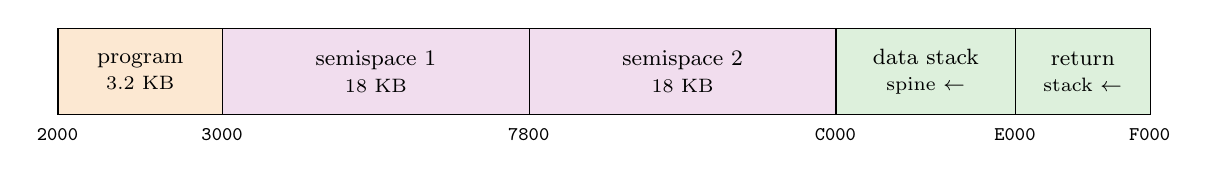
\begin{tikzpicture}[x=0.95cm]
\foreach \a/\b/\t/\f in {0/2.2/{program\\\scriptsize 3.2 KB}/cfill,
                         2.2/6.3/{semispace 1\\\scriptsize 18 KB}/hfill,
                         6.3/10.4/{semispace 2\\\scriptsize 18 KB}/hfill,
                         10.4/12.8/{data stack\\\scriptsize spine $\leftarrow$}/sfill,
                         12.8/14.6/{return\\\scriptsize stack $\leftarrow$}/sfill}
  \node[draw, fill=\f, minimum height=1.1cm, minimum width=(\b-\a)*0.95cm, anchor=west,
        align=center, inner sep=1pt, font=\footnotesize] at (\a,0) {\t};
\foreach \a/\t in {0/2000, 2.2/3000, 6.3/7800, 10.4/C000, 12.8/E000, 14.6/F000}
  \node[font=\scriptsize\ttfamily, anchor=north] at (\a,-0.6) {\t};
\end{tikzpicture}
\caption{Memory layout of \texttt{graph.asm}, not to scale. The heap is two
semispaces of 4,608 cells each. The spine grows down from \texttt{0xE000};
the machine stops with ``out of stack'' before it reaches the heap.}
\label{fig:memory}
\end{figure}

\subsection{The compiler}

The reader builds the syntax tree in the heap, out of the same two-word
cells. The compiler then works through it recursively:

\begin{itemize}[itemsep=2pt]
\item A leaf is left alone.
\item An application is compiled in place: its two halves are compiled and
  stored back into the same cell.
\item A $\lambda$-cell $(\lambda x, M)$ is replaced by $\abs{x}{M'}$, where
  $M'$ is the compiled body. The abstraction is a recursive procedure that
  follows the three basic rules, with each $\Sc$ built by a procedure that
  applies Turner's simplifications in the order of \cref{sec:turner}.
\end{itemize}

\noindent
Finally the compiled term is checked for variables: any variable left over
was not bound by a $\lambda$, and is reported as unbound. Turner's rules need
only a look at the first two levels of their arguments, to recognise
$\K\,p$, $\I$, and $\B\,p\,q$, so the whole compiler is about 150 instructions of
VM16 assembly.

\subsection{The reducer}

The reducer is a procedure, \texttt{whnf}, that reduces the graph at a given
cell to WHNF. Its spine is the VM16 data stack, and register \texttt{r9}
remembers where the current spine began, so that nested calls (for $\IF$ and
the operators) stack their spines on top of each other. Unwinding is a short
loop:
\begin{lstlisting}
unwind: LI      r1, 1
        AND     r1, r0
        BNZ     r1, wh_number           ; an odd word: a number
        BLTU    r0, r14, wh_comb        ; below the heap: a combinator
        PUSH    r0                      ; a cell: push it on the spine,
        GETDSP  r1
        BLTU    r1, r13, wh_full        ; (unless the stack is full)
        LW      r0, [r0]                ; and go down its function half
        JMP     unwind
\end{lstlisting}
At a combinator, the reducer compares the number of cells on the spine with
the combinator's number of arguments, from a table, and either stops (a
partial application) or jumps to the rule through another table. Each rule
reads its arguments from the argument halves of the spine cells. This is
the $\Sc$ rule:
\begin{lstlisting}
r_s:    BGEU    r11, r10, rs_go         ; S f g x = f x (g x)
        CALL    collect                 ; (make room for 3 cells first)
rs_go:  GETDSP  r7
        LW      r1, [r7]
        LW      r1, [r1+2]              ; f
        LW      r2, [r7+2]
        LW      r2, [r2+2]              ; g
        LW      r0, [r7+4]              ; the root
        LW      r3, [r0+2]              ; x
        SW      r1, [r10]               ; a new cell (f x)
        SW      r3, [r10+2]
        SW      r10, [r0]               ; overwrite the root's function
        ADDI    r10, CELL
        SW      r2, [r10]               ; a new cell (g x)
        SW      r3, [r10+2]
        SW      r10, [r0+2]             ; overwrite the root's argument
        ADDI    r10, CELL
        ADDI    r7, 6                   ; pop the three spine cells
        SETDSP  r7
        JMP     unwind                  ; and unwind from the root
\end{lstlisting}
Register \texttt{r10} is the allocation pointer, and \texttt{r11} the end of
the semispace minus three cells, so one comparison decides whether a rule
can allocate without collecting. The $\Y$ rule is four instructions:
\begin{lstlisting}
r_y:    POP     r0                      ; the root, Y f
        LW      r1, [r0+2]              ; f
        SW      r1, [r0]                ; the root becomes f ...
        SW      r0, [r0+2]              ; ... applied to the root itself
        JMP     unwind
\end{lstlisting}
The reducer, its rules and the arithmetic take about 940 bytes.

\subsection{Garbage collection}

The heap is managed by Cheney's copying collector~\cite{cheney70}: when the
current semispace is full, every cell reachable from the \emph{roots} is
copied to the other semispace, and the two swap roles. Finding the roots is
easy here, because the data stack holds every live pointer:

\begin{itemize}[itemsep=2pt]
\item \textbf{The spine is the root set.} Everything the program still needs
  is reachable from some cell on some spine, including the spines of
  suspended outer calls of \texttt{whnf}. The data stack also holds a few
  words that are not cells: saved spine bases, which are stack addresses,
  numbers, and rule addresses for the operators. None of them lies inside
  the heap, so the collector can safely leave them alone.
\item \textbf{Room before reading.} A rule that allocates first checks that
  three cells are free, collecting if not, and only then reads its arguments
  from the spine. So no rule ever holds a heap pointer in a register across a
  collection, which would leave it pointing at the old copy.
\item \textbf{Reloading after nesting.} $\IF$ and the operators call
  \texttt{whnf} on an argument, during which a collection may move
  everything. Afterwards they read the spine again rather than relying on
  registers.
\end{itemize}

\noindent
The forwarding address of a copied cell is marked by storing 0, which is not
a valid combinator, in its function half. Cycles made by $\Y$ need no special
care: Cheney's algorithm copies each cell exactly once.

% =====================================================================
\section{Measurements}\label{sec:measure}

\Cref{tab:measure} compares the graph reducer with the SECD machine and the
CAM of the companion tutorials, both also written in VM16 assembly. The
measure is the number of VM16 instructions executed, counted by the C
interpreter, which is independent of the host.

\begin{table}[t]
\centering
\small
\begin{tabular}{@{}l l r r r@{}}
\toprule
program & machine & machine steps & collections & VM16 instructions\\
\midrule
$\mathit{fac}\ 7$, \textbf{rec} & CAM & 171 instructions & 0 & 10,131\\
 & graph & 90 reductions & 0 & 14,717\\
\midrule
$\mathit{fac}\ 7$, with $Z$ & SECD & 322 transitions & 0 & 29,738\\
 & CAM & 346 instructions & 0 & 17,595\\
 & graph & 151 reductions & 0 & 23,848\\
\midrule
$\mathit{fib}(20)$ & SECD, with $Z$ & --- & 702 & 61,161,761\\
 & CAM, \textbf{rec} & 448,762 instructions & 16 & 7,035,081\\
 & graph, \textbf{rec} & 240,800 reductions & 46 & 16,808,595\\
 & VM16 assembly & --- & --- & 175,169\\
\midrule
$5!$, Church numerals & SECD & 52,044 transitions & 49 & 4,086,035\\
 & CAM & 73,681 instructions & 10 & 1,505,151\\
 & graph & 16,987 reductions & 2 & 968,914\\
\midrule
$5!$, Church, with $\Y$ (\texttt{church.lam}) & graph only & 16,957 reductions & 2 & 961,028\\
100th prime (\texttt{primes.lam}) & graph only & 155,171 reductions & 43 & 10,775,359\\
\bottomrule
\end{tabular}
\caption{The same programs on the three machines. The VM16 counts include
reading and compiling the program. The Church numeral program is
\texttt{fac.lam} from the SECD tutorial, with its $Z$ combinator and thunks,
so that all three machines can run it.}
\label{tab:measure}
\end{table}

\begin{figure}[t]
\centering
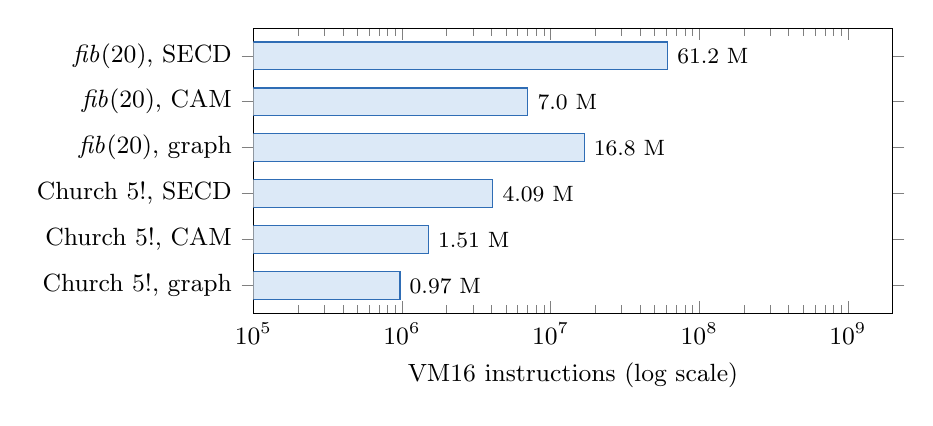
\begin{tikzpicture}
\begin{axis}[xbar, width=0.8\textwidth, height=5.2cm, xmode=log,
  xmin=1e5, xmax=2e9, log basis x=10,
  symbolic y coords={fib SECD, fib CAM, fib graph, Church SECD, Church CAM, Church graph},
  ytick=data, yticklabels={{$\mathit{fib}(20)$, SECD}, {$\mathit{fib}(20)$, CAM}, {$\mathit{fib}(20)$, graph},
    {Church $5!$, SECD}, {Church $5!$, CAM}, {Church $5!$, graph}},
  y dir=reverse, bar width=0.35cm, enlarge y limits=0.12,
  xlabel={VM16 instructions (log scale)},
  nodes near coords, nodes near coords align={horizontal},
  every node near coord/.append style={font=\footnotesize, anchor=west},
  point meta=explicit symbolic]
\addplot[fill=tfill, draw=tline] coordinates {
  (61161761,fib SECD) [61.2 M]
  (7035081,fib CAM) [7.0 M]
  (16808595,fib graph) [16.8 M]
  (4086035,Church SECD) [4.09 M]
  (1505151,Church CAM) [1.51 M]
  (968914,Church graph) [0.97 M]};
\end{axis}
\end{tikzpicture}
\caption{Two kinds of program. On $\mathit{fib}$, which is first-order
arithmetic, the CAM is 2.4 times faster than the graph reducer. On Church
numerals, which are nothing but higher-order functions, the graph reducer is
the fastest, 1.6 times faster than the CAM.}
\label{fig:bars}
\end{figure}

\paragraph{First-order programs.} On $\mathit{fac}$ and $\mathit{fib}$, the
graph reducer takes fewer steps than the CAM, but each step costs more:
about 70 VM16 instructions per reduction against 16 per CAM instruction. On
$\mathit{fib}(20)$ that makes it 2.4 times slower than the CAM, though still
3.6 times faster than the SECD machine. \Cref{tab:mix} shows where the
reductions go. Each call of $\mathit{fib}$ takes 11 reductions, and only
three of them do arithmetic; the rest move $n$ and $f$ to where they are
needed. $\C$ and $\I$ alone are 36\,\% of the work.

\begin{table}[t]
\centering
\small
\begin{tabular}{@{}l r r r@{}}
\toprule
rule & reductions & per call & share\\
\midrule
$\C$ & 43,783 & 2 & 18.2\,\%\\
$\I$ & 43,780 & 2 & 18.2\,\%\\
$\Sc$ & 32,836 & 1.5 & 13.6\,\%\\
$\Sp$ & 21,892 & 1 & 9.1\,\%\\
$\IF$ & 21,891 & 1 & 9.1\,\%\\
${<}$ & 21,891 & 1 & 9.1\,\%\\
${-}$ & 21,890 & 1 & 9.1\,\%\\
$\B$ & 10,946 & 0.5 & 4.5\,\%\\
$\Bs$ & 10,945 & 0.5 & 4.5\,\%\\
${+}$ & 10,945 & 0.5 & 4.5\,\%\\
$\Y$ & 1 & & \\
\midrule
total & 240,800 & 11 & \\
\bottomrule
\end{tabular}
\caption{The reductions in $\mathit{fib}(20)$, which makes 21,891 calls,
from \texttt{prototype.py -{}-counts}. Half the calls are leaves ($n < 2$),
which do not add.}
\label{tab:mix}
\end{table}

The 70 instructions per reduction break down roughly as follows. Unwinding
pushes 2.5 cells per reduction on average, at 9 instructions each, about 25
in all; checking the number of arguments and dispatching through the table
takes 13; and the rule itself takes the rest, between 4 for $\Y$ and about
30 for the operators, which also call \texttt{whnf} on their arguments.

\paragraph{Higher-order programs.} On Church numerals the picture reverses.
The graph reducer needs 16,987 reductions where the CAM needs 73,681
instructions, and it is 1.6 times faster than the CAM and 4.2 times faster
than the SECD machine. Church numerals are functions that apply other
functions many times. The CAM and the SECD machine build a closure and an
environment for every application, while a combinator rule only rearranges
the pointers it was given. Sharing helps too: a numeral that is used several
times is built once.

\paragraph{Turner's combinators.} \Cref{tab:sizes} shows what the extra
combinators of \cref{sec:turner} are worth. They make the code 2.5 to 6
times smaller, and the programs 2.3 to 13 times faster, the most on the
biggest program, where the plain $\Sc$ rule passes arguments down long paths
that never use them.

\begin{table}[t]
\centering
\small
\begin{tabular}{@{}l r r r r@{}}
\toprule
 & \multicolumn{2}{c}{code (cells)} & \multicolumn{2}{c}{reductions}\\
\cmidrule(lr){2-3}\cmidrule(l){4-5}
program & $\Sc\,\K\,\I$ & Turner & $\Sc\,\K\,\I$ & Turner\\
\midrule
\texttt{fac.lam} & 40 & 16 & 216 & 90\\
\texttt{fib.lam} & 57 & 22 & 547,279 & 240,800\\
\texttt{church.lam} & 540 & 98 & 47,967 & 16,957\\
\texttt{primes.lam} & 602 & 107 & 2,047,673 & 155,171\\
\bottomrule
\end{tabular}
\caption{Code size and reductions with $\Sc$, $\K$, $\I$ only (plus the
$\K$ simplification), and with Turner's rules, from \texttt{prototype.py}
with and without \texttt{-{}-ski}.}
\label{tab:sizes}
\end{table}

\paragraph{On a Z80.} The Z80 VM16 interpreter averages about 288 clock
cycles per VM16 instruction on this program. At 4\,MHz, $\mathit{fac}\ 7$ takes
1.1 seconds and the Church factorial 72 seconds, both measured on a Z80
emulator, and $\mathit{fib}(20)$ would take about 20 minutes.

% =====================================================================
\section{Variations and descendants}\label{sec:descendants}

\begin{description}[style=nextline, leftmargin=1.2em, itemsep=3pt]
\item[Hardware.] SKIM, the S, K, I reduction machine built at
  Cambridge~\cite{skim80}, ran combinator code directly in microcode, and
  later projects such as NORMA explored the idea further. Graph reduction
  turned out to run well enough on ordinary processors, and special hardware
  did not catch on.
\item[Supercombinators.] Turner's combinators are fixed, so a program needs
  many small steps. Hughes~\cite{hughes82} proposed instead to turn each
  function of the program into its own combinator, a \emph{supercombinator},
  by lifting out its free variables. One reduction then does the work of a
  whole function body.
\item[The G-machine.] Johnsson and Augustsson compiled each supercombinator
  into code for an abstract machine that builds and rewrites the graph, the
  G-machine~\cite{johnsson84,augustsson84}, and from there to native code.
  That was the basis of the Lazy ML compiler and of the textbook by Peyton
  Jones~\cite{spj87}, which remains the best introduction to the whole area,
  together with its practical companion~\cite{spjlester92}.
\item[The STG machine.] GHC, the main Haskell compiler, still reduces graphs,
  but its Spineless Tagless G-machine~\cite{spj92} avoids building the spine
  as a separate structure and represents every node as code that knows how
  to evaluate itself.
\item[Combinators again.] Bracket abstraction itself has never gone away.
  Kiselyov~\cite{kiselyov18} gives algorithms whose code size grows linearly
  with the program, and Augustsson's MicroHs, a small Haskell implementation,
  compiles Haskell to combinators and runs them on a graph reducer, much as
  Turner did.
\end{description}

% =====================================================================
\section{Summary}

Combinator graph reduction removes the variables from a program before
running it. Bracket abstraction translates each $\lambda x.M$ into a term built
from a fixed set of combinators, using the rules $\abs{x}{x} = \I$,
$\abs{x}{e} = \K\,e$ and $\abs{x}{(e_1\,e_2)} = \Sc\,(\abs{x}{e_1})\,(\abs{x}{e_2})$,
and Turner's extra combinators $\B$, $\C$, $\Sp$, $\Bs$, $\Cp$ keep the result
small. The machine then needs no environments and no closures. It unwinds the
spine to find the leftmost outermost redex, rewrites the root of the redex in
place according to the combinator's rule, and repeats. Because arguments are
shared and roots are overwritten, every expression is reduced at most once and
only when needed, which is lazy evaluation. $\Y$ becomes a cycle, $\IF$ needs
no thunks, and infinite lists come for free. The machine is small and
regular, its only garbage-collection roots are the cells on the spine, and in
our measurements it is the fastest of the three machines on higher-order
programs and 2.4 times slower than the CAM on first-order arithmetic.

% =====================================================================
\section*{Exercises}
\addcontentsline{toc}{section}{Exercises}

\begin{exercise}
Compile $\lambda f\,g\,x.\,f\,(g\,x)$ by hand, first with the three basic
rules and then with Turner's. Check your answer by running
\verb|echo '? \f g x.f (g x)' | ../vm16 graph.v16|. Do the same for
$\lambda f\,x\,y.\,f\,y\,x$.
\end{exercise}

\begin{exercise}
Extend the proof of \cref{thm:abs} to Turner's rules: show that each
simplification of \cref{sec:turner} preserves the property
$(\abs{x}{e})\,x \reds e$. Which of them relies on $\eta$-conversion, and why
is that harmless for a program that is only run, never compared?
\end{exercise}

\begin{exercise}
Trace $(\lambda x\,y.\,y\,x)\;3\;(\lambda z.\,{*}\;z\;z)$ by hand. It compiles
to $\C\,\I\,3\,(\Sc\,{*}\,\I)$ and takes 5 reductions. Check with
\texttt{prototype.py -{}-trace}. Where is the 3 shared?
\end{exercise}

\begin{exercise}
The rules overwrite the \emph{root} of a redex. Suppose an implementation
built a fresh cell for the result instead and left the root alone. Find a
program for which it computes the same result but does more reductions, and
explain why. What property of the program decides how much is lost?
\end{exercise}

\begin{exercise}\label{ex:seq}
Add a combinator $\cmb{SEQ}$ with the rule $\cmb{SEQ}\,a\,b \red b$, after
reducing $a$ to WHNF, and a source form \texttt{seq a b} for it. Use it to fix
the space leak of \cref{sec:leaks}. How many reductions does the loop take
for $n = 3000$?
\end{exercise}

\begin{exercise}
After every rewrite, the reducer pops the redex and unwinds again from its
root, pushing the root again. For which rules is the new head of the root
known without unwinding? Estimate from \cref{tab:mix} how many of the 70
instructions per reduction this would save in $\mathit{fib}(20)$.
\end{exercise}

\begin{exercise}
The reducer checks for stack overflow on every push. Show that it would be
enough to check once per reduction and at every nested call of
\texttt{whnf}, provided the check leaves room for a bounded number of pushes.
What is the bound, and why does it depend on the program?
\end{exercise}

\begin{exercise}
$\mathbf{rec}\ x.\,x$ is detected because the indirection points to itself.
$\mathbf{rec}\ x.\,{+}\;x\;1$ is just as meaningless, but the check does not
catch it: the machine nests deeper and deeper until it runs out of stack.
Explain why. GHC handles such cases with \emph{black holes}: a cell is marked
when its evaluation starts, and reaching a marked cell is an error. Design
that for \texttt{graph.asm}. Which cells need marking?
\end{exercise}

\begin{exercise}
Write $\mathit{map}$, $\mathit{take}$ and $\mathit{sum}$ for the list
encoding of \cref{sec:laziness}, and use them to compute the sum of the
squares of the first 20 primes. Is the sum reduced before or after the
primes are generated?
\end{exercise}

\begin{exercise}
Turner's languages did input and output with lazy lists: the program is a
function from the input characters to the output characters. Design a
version of \texttt{graph.asm} that prints the elements of a result list as
they are produced, so that \texttt{primes.lam} could print primes forever.
Which parts of the reducer change, and which roots must the collector know
about?
\end{exercise}

% =====================================================================
\section{Reference card}\label{sec:card}

\begin{center}
\small
\renewcommand{\arraystretch}{1.15}
\begin{tabular}{@{}l l@{}}
\toprule
\multicolumn{2}{@{}l}{\textbf{Bracket abstraction} \quad (compile the body of each $\lambda x.M$ first, then abstract $x$)}\\
\midrule
$\abs{x}{x} = \I$ & $\abs{x}{e} = \K\,e$ \ (any other leaf)\\
$\abs{x}{(e_1\,e_2)} = \Sc\,(\abs{x}{e_1})\,(\abs{x}{e_2})$, simplified: & \\
\quad $\Sc\,(\K\,p)\,(\K\,q) = \K\,(p\,q)$ & \quad $\Sc\,(\B\,p\,q)\,(\K\,r) = \Cp\,p\,q\,r$\\
\quad $\Sc\,(\K\,p)\,\I = p$ & \quad $\Sc\,p\,(\K\,q) = \C\,p\,q$\\
\quad $\Sc\,(\K\,p)\,(\B\,q\,r) = \Bs\,p\,q\,r$ & \quad $\Sc\,(\B\,p\,q)\,r = \Sp\,p\,q\,r$\\
\quad $\Sc\,(\K\,p)\,q = \B\,p\,q$ & \\
$\mathbf{if}\ c\ t\ e = \IF\,c\,t\,e$ & $\mathbf{rec}\ f.M = \Y\,(\lambda f.M)$\\
\midrule
\multicolumn{2}{@{}l}{\textbf{Rules} \quad (the root of the redex is overwritten; $\to \I\,v$ means an indirection)}\\
\midrule
$\I\,x \red x$ & $\Y\,f \red f\,(\Y\,f)$, as a cycle\\
$\K\,x\,y \red x$ & $\Sp\,k\,f\,g\,x \red k\,(f\,x)\,(g\,x)$\\
$\Sc\,f\,g\,x \red f\,x\,(g\,x)$ & $\Bs\,k\,f\,g\,x \red k\,(f\,(g\,x))$\\
$\B\,f\,g\,x \red f\,(g\,x)$ & $\Cp\,k\,f\,g\,x \red k\,(f\,x)\,g$\\
$\C\,f\,g\,x \red f\,x\,g$ & $\IF\,c\,t\,e \red t$ (if $c \ne 0$) or $e$, reducing $c$ first\\
\multicolumn{2}{@{}l}{${+}\,a\,b \red a+b$, reducing $a$ and $b$ first; likewise ${-}$ ${*}$ ${/}$ ${\%}$, and ${=}$, ${<}$ giving 1 or 0}\\
\midrule
\multicolumn{2}{@{}l}{\textbf{Machine}}\\
\midrule
\multicolumn{2}{@{}l}{Unwind: from the root, push each cell and follow its function half, until a leaf.}\\
\multicolumn{2}{@{}l}{A combinator with $n$ arguments and $\ge n$ cells on the spine: rewrite the $n$th cell, pop $n$, unwind from it.}\\
\multicolumn{2}{@{}l}{Fewer cells: WHNF, a partial application. A number with an empty spine: the result.}\\
\bottomrule
\end{tabular}
\end{center}

% =====================================================================
\begin{thebibliography}{99}
\small

\bibitem{augustsson84}
L.~Augustsson.
\newblock A compiler for lazy {ML}.
\newblock In \emph{ACM Symposium on LISP and Functional Programming}, pages
  218--227, 1984.

\bibitem{cam87}
G.~Cousineau, P.-L. Curien, and M.~Mauny.
\newblock The categorical abstract machine.
\newblock \emph{Science of Computer Programming}, 8(2):173--202, 1987.

\bibitem{cheney70}
C.~J. Cheney.
\newblock A nonrecursive list compacting algorithm.
\newblock \emph{Communications of the ACM}, 13(11):677--678, 1970.

\bibitem{skim80}
T.~J.~W. Clarke, P.~J.~S. Gladstone, C.~D. MacLean, and A.~C. Norman.
\newblock {SKIM} --- the {S}, {K}, {I} reduction machine.
\newblock In \emph{ACM Conference on LISP and Functional Programming}, pages
  128--135, 1980.

\bibitem{curryfeys58}
H.~B. Curry and R.~Feys.
\newblock \emph{Combinatory Logic}, volume~I.
\newblock North-Holland, 1958.

\bibitem{hughes82}
R.~J.~M. Hughes.
\newblock Super-combinators: a new implementation method for applicative
  languages.
\newblock In \emph{ACM Symposium on LISP and Functional Programming}, pages
  1--10, 1982.

\bibitem{johnsson84}
T.~Johnsson.
\newblock Efficient compilation of lazy evaluation.
\newblock In \emph{SIGPLAN Symposium on Compiler Construction}, pages 58--69,
  1984.

\bibitem{kiselyov18}
O.~Kiselyov.
\newblock $\lambda$ to {SKI}, semantically.
\newblock In \emph{Functional and Logic Programming (FLOPS)}, volume 10818 of
  \emph{LNCS}, pages 33--50. Springer, 2018.

\bibitem{landin64}
P.~J. Landin.
\newblock The mechanical evaluation of expressions.
\newblock \emph{The Computer Journal}, 6(4):308--320, 1964.

\bibitem{spj87}
S.~L. Peyton~Jones.
\newblock \emph{The Implementation of Functional Programming Languages}.
\newblock Prentice Hall, 1987.

\bibitem{spj92}
S.~L. Peyton~Jones.
\newblock Implementing lazy functional languages on stock hardware: the
  {S}pineless {T}agless {G}-machine.
\newblock \emph{Journal of Functional Programming}, 2(2):127--202, 1992.

\bibitem{spjlester92}
S.~L. Peyton~Jones and D.~R. Lester.
\newblock \emph{Implementing Functional Languages: a Tutorial}.
\newblock Prentice Hall, 1992.

\bibitem{schonfinkel24}
M.~Schönfinkel.
\newblock Über die {B}austeine der mathematischen {L}ogik.
\newblock \emph{Mathematische Annalen}, 92:305--316, 1924.

\bibitem{turner79}
D.~A. Turner.
\newblock A new implementation technique for applicative languages.
\newblock \emph{Software---Practice and Experience}, 9(1):31--49, 1979.

\bibitem{turner79b}
D.~A. Turner.
\newblock Another algorithm for bracket abstraction.
\newblock \emph{Journal of Symbolic Logic}, 44(2):267--270, 1979.

\end{thebibliography}

\end{document}
